\scanpage{15}\mspage{14}
In summary, in terms of $\unsure{\mathcal{F}|\mathfrak{F}}$, it is from the datum of two \uline{order} \uline{relations}
% The enclosure has separate top, left and bottom strokes; no right vertical is visible.
\figure{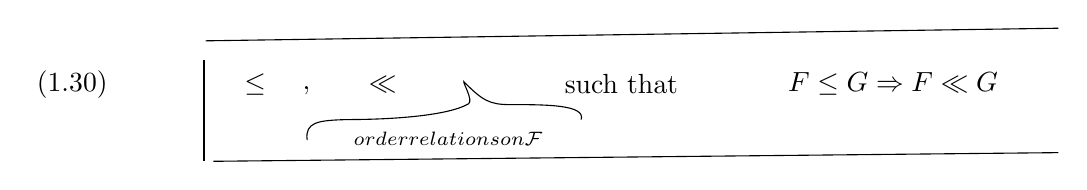
\begin{tikzpicture}[x=1cm,y=1cm]
  \node[anchor=east] at (-1.1,0.68) {$(1.30)$};
  \node at (0.65,0.68) {$\leq$};
  \node at (1.30,0.59) {$,$};
  \node at (2.27,0.68) {$\ll$};
  \node at (5.30,0.68) {such that};
  \node at (8.75,0.68) {$F\leq G\Rightarrow F\ll G$};
  \node at (3.10,-0.02) {$\scriptstyle\text{order relations on }\mathcal{F}$};
  \draw (0.02,1.23) -- (10.85,1.39);
  \draw (0,0.99) -- (0,-0.30);
  \draw (0.12,-0.30) -- (10.85,-0.19);
  \draw (1.31,-0.03) .. controls (1.28,0.20) and (1.45,0.22) .. (1.82,0.23)
    .. controls (2.40,0.23) and (3.10,0.28) .. (3.36,0.43)
    .. controls (3.42,0.48) and (3.29,0.69) .. (3.30,0.71)
    .. controls (3.53,0.48) and (3.62,0.42) .. (3.88,0.42)
    .. controls (4.34,0.42) and (4.85,0.42) .. (4.79,0.23);
\end{tikzpicture}}
that I am going to start.

In terms of these, one defines \deleted{$\unsure{\mathcal{M}|M}$}
\[
\mathcal{M}\subset\mathcal{F}
\]
by (1.20), \unsure{with} the relations $\underset{\mathcal{M}}{\leq},\ \underset{\mathcal{M}}{\ll}$ induced by $\underset{\mathcal{F}}{\leq},\ \underset{\unsure{\mathcal{F}|\overline{f}}}{\ll}$, then
\[
\mathcal{L}\subset\mathcal{M}
\]
by (1.25). The map
\[
\mathcal{F}\hookrightarrow\unsure{\mathcal{P}|\mathscr{P}|\mathfrak{P}}(\mathcal{M})\qquad
\mathord{\rlap{$\deleted{X}$}F}\longmapsto\widetilde F=\mathrm{Dep}(F)
\tag*{($*$)}
\]
% The input X is overwritten by F at the same horizontal position.
is \inserted{then} defined by
\[
\widetilde F=\{X\in\mathcal{M}\mid X\leq F\}
\tag*{(1.31)}
\]
and
\[
\mathcal{F}\hookrightarrow\mathrm{Fig}(\mathcal{M})\qquad
\unsure{F|\deleted{F}|\mathord{\rlap{$\deleted{X}$}F}}\longmapsto\mathrm{Fig}_{\mathcal{M}}(F)
\tag*{($**$)}
\]
% At the second map an extra diagonal crosses F; live F, canceled F, and X overwritten by F remain possible.
by (1.4) :
\[
\mathrm{Fig}_{\mathcal{M}}(F)=\{\widetilde X\mid X\in\widetilde F\}\subset\mathcal{P}(\mathcal{M})
\tag*{\deleted{(1.32)}}
\]
with
\[
\widetilde X=\{Y\in\mathcal{M}\mid Y\leq X\}\quad.
\]

Thus, $\mathcal{F}$ is interpreted as a set of subsets of $\mathcal{M}$ via ($*$), and $\leq$ \unsure{is interpreted|is interpreted} simply by inclusion
\[
F\leq G\Longleftrightarrow\widetilde F\subset\widetilde G
\tag*{(1.32)}
\]
